\documentclass{Article}
\usepackage[utf8]{inputenc}
\usepackage [danish]{babel}
\usepackage[a4paper, hmargin={2.8cm, 2.8cm}, vmargin={2.5cm, 2.5cm}]{geometry}
\usepackage{eso-pic} % \AddToShipoutPicture
\usepackage{graphicx} % \includegraphics
\linespread{1.2}
\usepackage{amsthm}
\usepackage{amsmath}
\usepackage{url}
\usepackage{tikz}
\usepackage{amsfonts}


\usepackage{listings}


\author{
\Large{dpj482}\\
    \\ \texttt{}
}

\title{
  \vspace{3cm}
  \Huge{CAC assignment 2} \\
  \Large{Christian Møllgaard}\\
}
\usepackage{natbib}
\usepackage{graphicx}

\begin{document}

%% Change `ku-farve` to `nat-farve` to use SCIENCE's old colors or
%% `natbio-farve` to use SCIENCE's new colors and logo.
%\AddToShipoutPicture*{\put(0,0){\includegraphics*[viewport=0 0 700 600]{natbio-farve}}}
\AddToShipoutPicture*{\put(0,602){\includegraphics*[viewport=0 600 700 1600]{natbio-farve}}}

%% Change `ku-en` to `nat-en` to use the `Faculty of Science` header
\AddToShipoutPicture*{\put(0,0){\includegraphics*{nat-en}}}

\clearpage\maketitle
\thispagestyle{empty}

%\newpage



%\lstinputlisting[language=Python, firstline=56, lastline=82]{nbodyphysics.py}

\section{Introduction}
The task of this assignment was to convert the given program to run in parallel on the same generated data. To do this the multiprocessing library is used together with the provided shared memory array shmarray class.

\section{What have changed}
\subsection*{Overall change}
As a first step i converted V and U to shared memory arrays using the shmarray library, and then made them global. This was needed to make sure the arrays could be called from within the new other processes. The main functions (RD and RD\_visual) then create a process pool. 

Then i divide U an V into cpu*2 pieces. Then i run the real RD function on each part seperatly and saving the result in another array called Ures and Vres. When all parts have been processes the result arrays are then copied into real array, and then the outer edges gets handled.

\subsection{The splitter}
Before any processing can be done, the data needs to be split up into a few pieces. I split the images based on 


\section{Result}



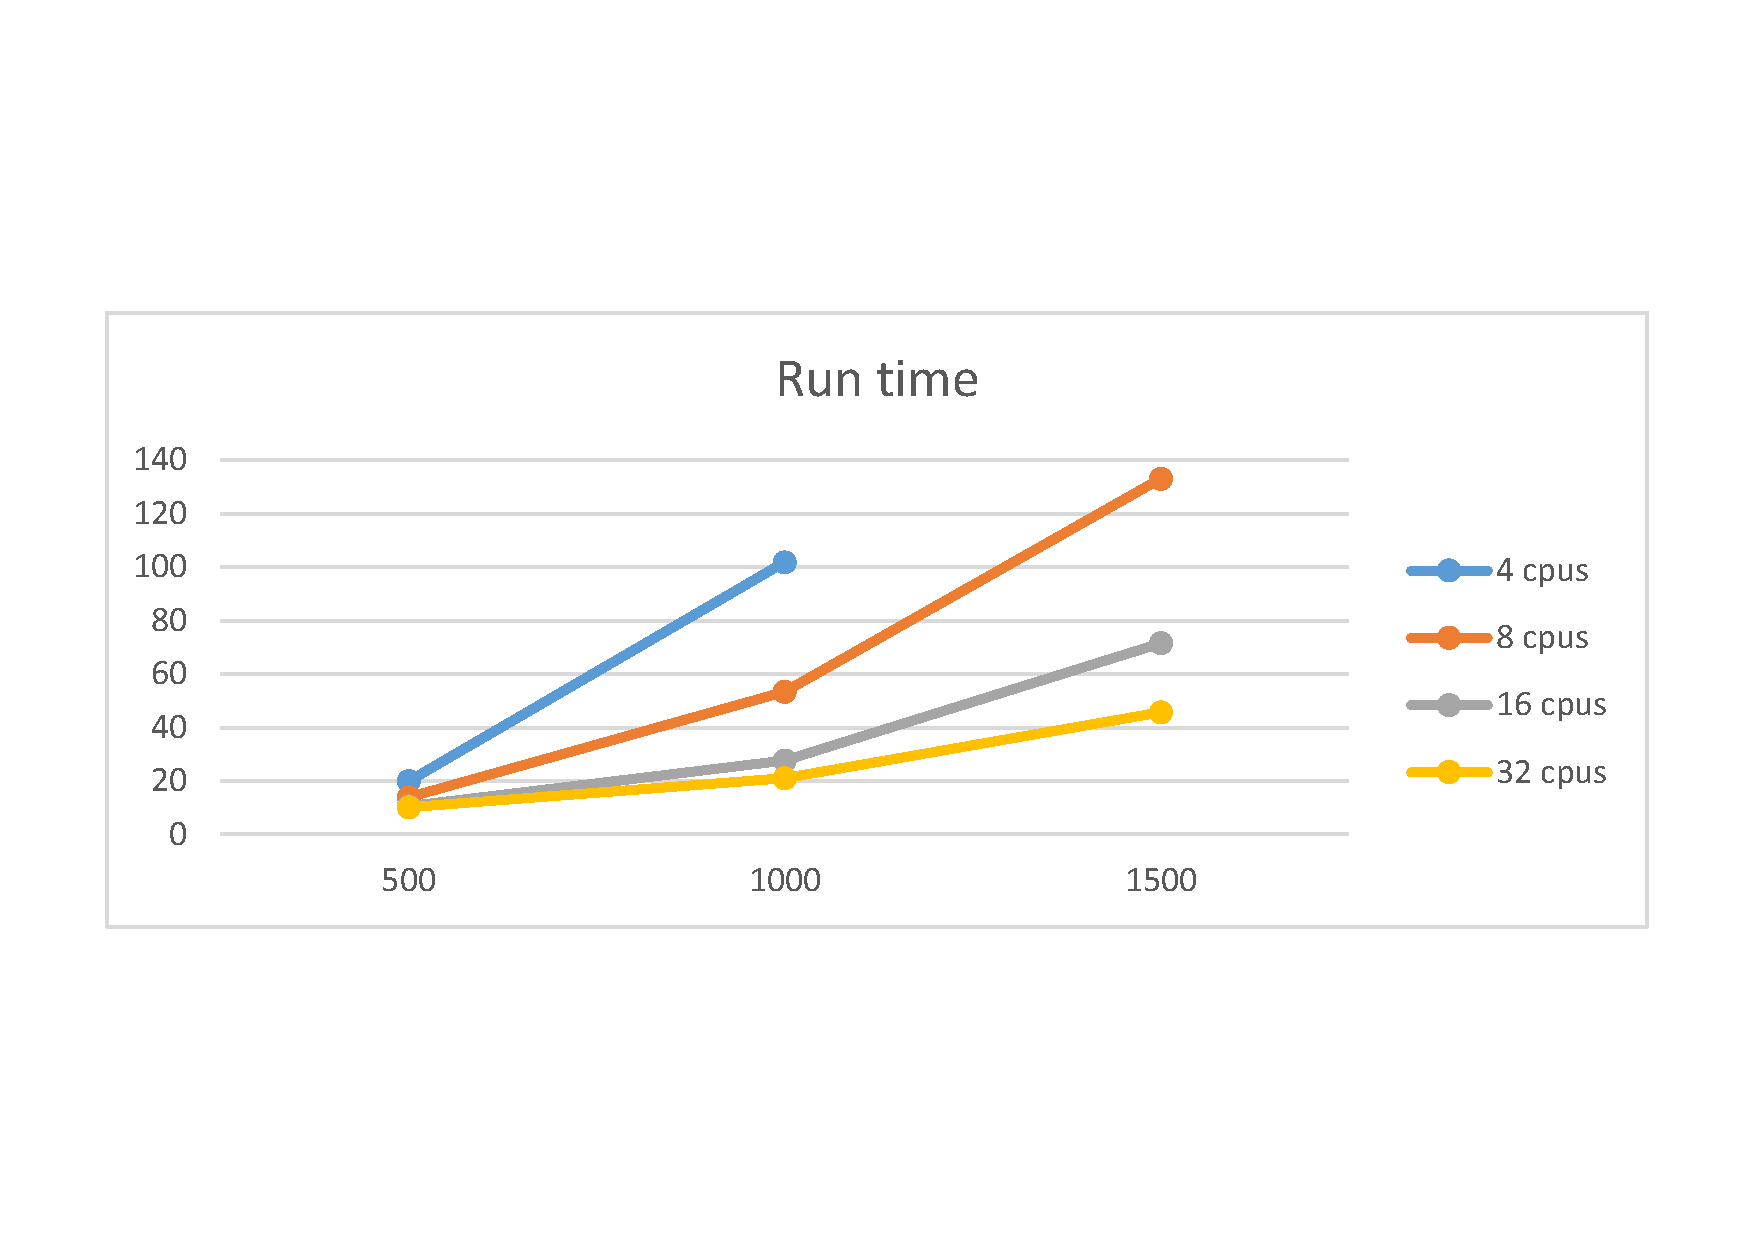
\includegraphics[scale=0.5]{plots}

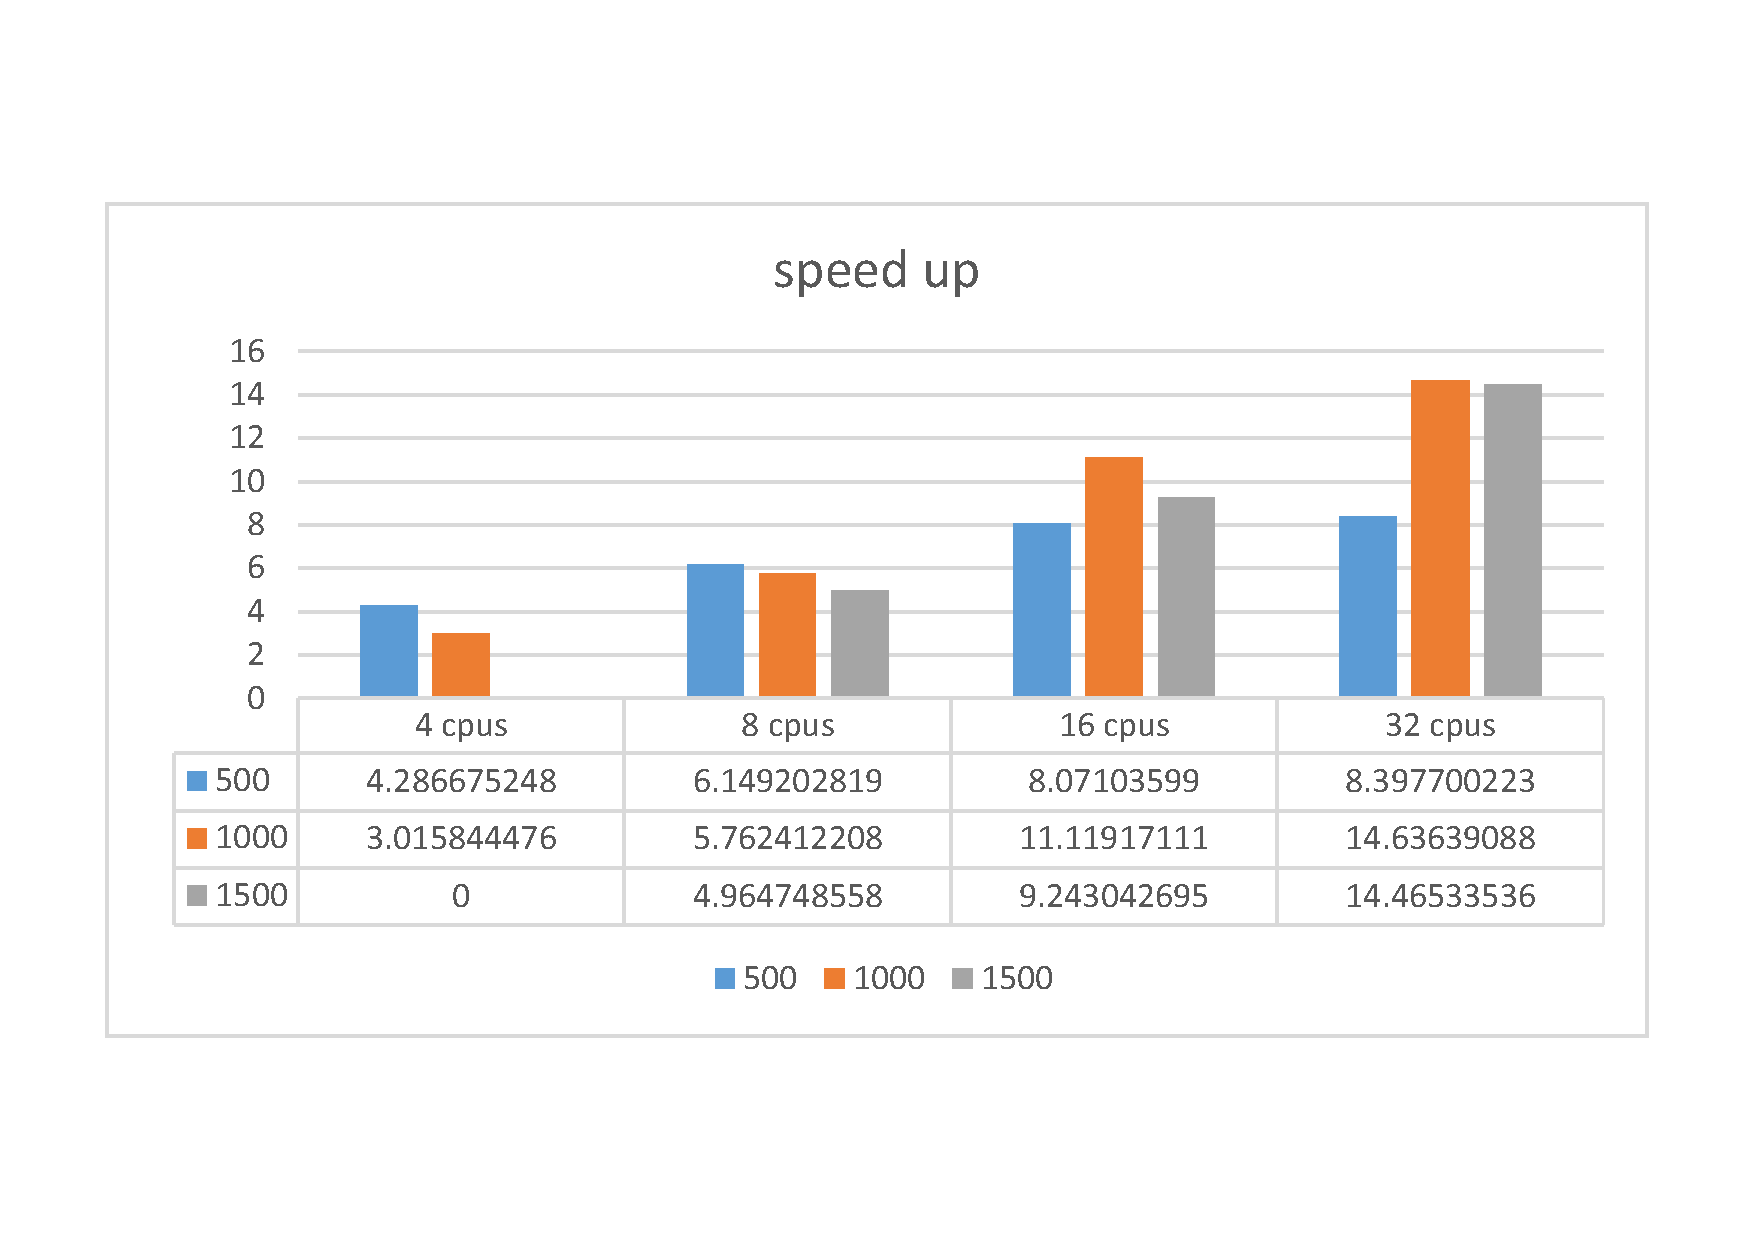
\includegraphics[scale=0.5]{speedup}

\end{document}
